% Presentacion final del proyecto KIWI (IS4024 DevOps).
% Version LaTeX/Beamer de docs/devsecops/entrega/Kiwi_Presentacion_Final.pdf,
% con el modelo STRIDE actualizado (diagramas/STRIDE.drawio: 17 amenazas,
% 7 fronteras, T1-T6 priorizadas) y el estado tras integrar los PR #11-#13.
% Compilar desde esta carpeta: pdflatex "Presentacion Final.tex" (dos veces).
\documentclass[aspectratio=169,11pt,xcolor=table]{beamer}

\usepackage[utf8]{inputenc}
\usepackage[T1]{fontenc}
\usepackage{lmodern}
\usepackage[spanish,provide=*]{babel}
\usepackage{graphicx}
\usepackage{booktabs,array,tabularx}
\usepackage{tikz}
\usepackage{pgfplots}
\pgfplotsset{compat=1.18}
\graphicspath{{images/}}

% Paleta tomada de la presentacion original.
\definecolor{navy}{RGB}{10,30,60}
\definecolor{cyan}{RGB}{18,160,225}
\definecolor{paper}{RGB}{238,246,252}
\definecolor{soft}{RGB}{214,236,250}
\definecolor{muted}{RGB}{90,105,125}
\definecolor{warn}{RGB}{252,226,226}
\definecolor{amber}{RGB}{253,236,200}
\definecolor{okgreen}{RGB}{220,242,224}

\newcolumntype{L}[1]{>{\raggedright\arraybackslash}p{#1}}
\newcolumntype{Y}{>{\raggedright\arraybackslash}X}

\setbeamertemplate{navigation symbols}{}
\setbeamercolor{background canvas}{bg=paper}
\setbeamercolor{normal text}{fg=navy}
\setbeamercolor{frametitle}{fg=navy}
\setbeamercolor{itemize item}{fg=cyan}
\setbeamertemplate{itemize item}[circle]
\setbeamerfont{frametitle}{series=\bfseries,size=\LARGE}

\newcommand{\utecbadge}{\colorbox{cyan}{\textcolor{white}{\footnotesize\bfseries\,UTEC\,}}}
\newcommand{\kicker}[1]{{\color{cyan}\scriptsize\bfseries\MakeUppercase{#1}}}

\setbeamertemplate{headline}{%
  \vskip6pt\hbox to\paperwidth{\hskip18pt\utecbadge\hfill
  {\color{muted}\tiny Kiwi · Informe final DevSecOps\quad\insertframenumber\,/\,\inserttotalframenumber}\hskip18pt}}
\setbeamertemplate{frametitle}{%
  \vskip4pt\kicker{\insertframesubtitle}\par\vskip1pt
  {\usebeamerfont{frametitle}\insertframetitle}\par}

% Tarjetas
\newcommand{\card}[3][paper]{% color de fondo, ancho, contenido
  \begin{tikzpicture}\node[fill=white,rounded corners=4pt,inner sep=8pt,text width=#2,
  draw=soft]{#3};\end{tikzpicture}}
\newcommand{\darkcard}[2]{%
  \begin{tikzpicture}\node[fill=navy,rounded corners=4pt,inner sep=10pt,text width=#1,
  text=white]{\setbeamercolor{normal text}{fg=white}\setbeamercolor{itemize/enumerate body}{fg=white}\color{white}#2};\end{tikzpicture}}
\newcommand{\stat}[3]{% ancho, numero, texto
  \begin{tikzpicture}\node[fill=white,draw=soft,rounded corners=4pt,inner sep=7pt,text width=#1]
  {{\color{navy}\LARGE\bfseries #2}\quad{\color{muted}\footnotesize #3}};\end{tikzpicture}}
\newcommand{\statdark}[3]{%
  \begin{tikzpicture}\node[fill=navy,rounded corners=4pt,inner sep=7pt,text width=#1]
  {{\color{cyan}\LARGE\bfseries #2}\quad{\color{white}\footnotesize #3}};\end{tikzpicture}}
\newcommand{\num}[1]{\tikz[baseline=(n.base)]\node[circle,fill=cyan,text=white,inner sep=2pt,
  minimum size=14pt,font=\scriptsize\bfseries](n){#1};}

\newenvironment{tabla}[1]{\renewcommand{\arraystretch}{1.3}\footnotesize
  \rowcolors{2}{white}{soft}\tabularx{\linewidth}{#1}}{\endtabularx}
\newcommand{\thead}[1]{\cellcolor{navy}\textcolor{white}{\bfseries #1}}

\begin{document}

% ---------------------------------------------------------------- 1. Portada
{
\setbeamercolor{background canvas}{bg=navy}
\setbeamertemplate{headline}{}
\begin{frame}[plain]
  \begin{tikzpicture}[remember picture,overlay]
    \fill[cyan] ([xshift=-2.2cm,yshift=-2.6cm]current page.north east) circle (1.6cm);
  \end{tikzpicture}
  \vskip10pt\utecbadge\vskip34pt
  {\color{white}\fontsize{44}{48}\selectfont\bfseries Kiwi}\par\vskip6pt
  {\color{cyan}\Large Informe final DevSecOps}\par\vskip40pt
  
\begin{tikzpicture}
    \node[fill=navy!70!cyan,rounded corners=5pt,inner sep=10pt,text width=0.9\paperwidth,text=white]{
      \scriptsize
      \begin{tabular}{@{}p{0.15\paperwidth}p{0.19\paperwidth}p{0.27\paperwidth}p{0.23\paperwidth}@{}}
        {\color{cyan}\tiny\bfseries CURSO} & {\color{cyan}\tiny\bfseries PROFESOR} &
        {\color{cyan}\tiny\bfseries EQUIPO} & {\color{cyan}\tiny\bfseries FECHA}\\
        IS4024 DevOps & Wilson Julca Mejía & Aarón Timaná Castro & 23 de noviembre de 2026\\
        & & Jean Piero Huaylla Huillca & \\
        & & Mateo Espinoza Monti & \\
      \end{tabular}};
  \end{tikzpicture}
\end{frame}
}

% ---------------------------------------------------------------- 2. Contexto
\begin{frame}{Problema educativo y alcance técnico}{Contexto del proyecto}
  \vskip6pt
  \begin{columns}[T]
    \column{0.36\textwidth}
    \darkcard{0.88\linewidth}{%
      {\color{cyan}\tiny\bfseries PROBLEMA EDUCATIVO}\par\vskip6pt
      {\large\bfseries Refuerzo de Comunicación para primero de secundaria}\par\vskip8pt
      {\scriptsize I.E. Fe y Alegría: acceso limitado a dispositivos.}}
    \column{0.6\textwidth}
    \card{0.92\linewidth}{\num{1}\enspace\small Docentes crean aulas y quizzes.}\par\vskip3pt
    \card{0.92\linewidth}{\num{2}\enspace\small Estudiantes practican y reciben recompensas.}\par\vskip3pt
    \card{0.92\linewidth}{\num{3}\enspace\small Gemini genera contenido a partir de texto o PDF.}\par\vskip3pt
    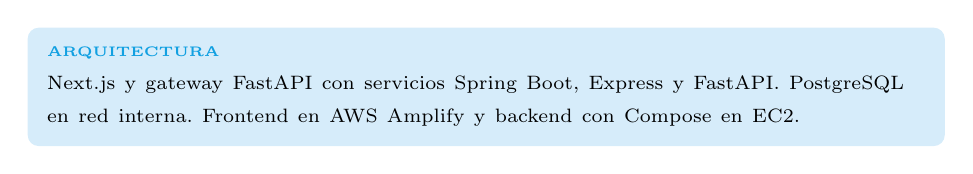
\begin{tikzpicture}\node[fill=soft,rounded corners=4pt,inner sep=7pt,text width=0.92\linewidth]{
      {\color{cyan}\tiny\bfseries ARQUITECTURA}\par
      \scriptsize Next.js y gateway FastAPI con servicios Spring Boot, Express y FastAPI.
      PostgreSQL en red interna. Frontend en AWS Amplify y backend con Compose en EC2.};
    \end{tikzpicture}
  \end{columns}
\end{frame}

% ---------------------------------------------------------------- 3. STRIDE
\begin{frame}{Modelo de amenazas STRIDE}{Modelo de amenazas}
  \vskip4pt
  \begin{columns}[T]
    \column{0.72\textwidth}
    \begin{tikzpicture}\node[fill=white,draw=soft,rounded corners=4pt,inner sep=4pt]{%
      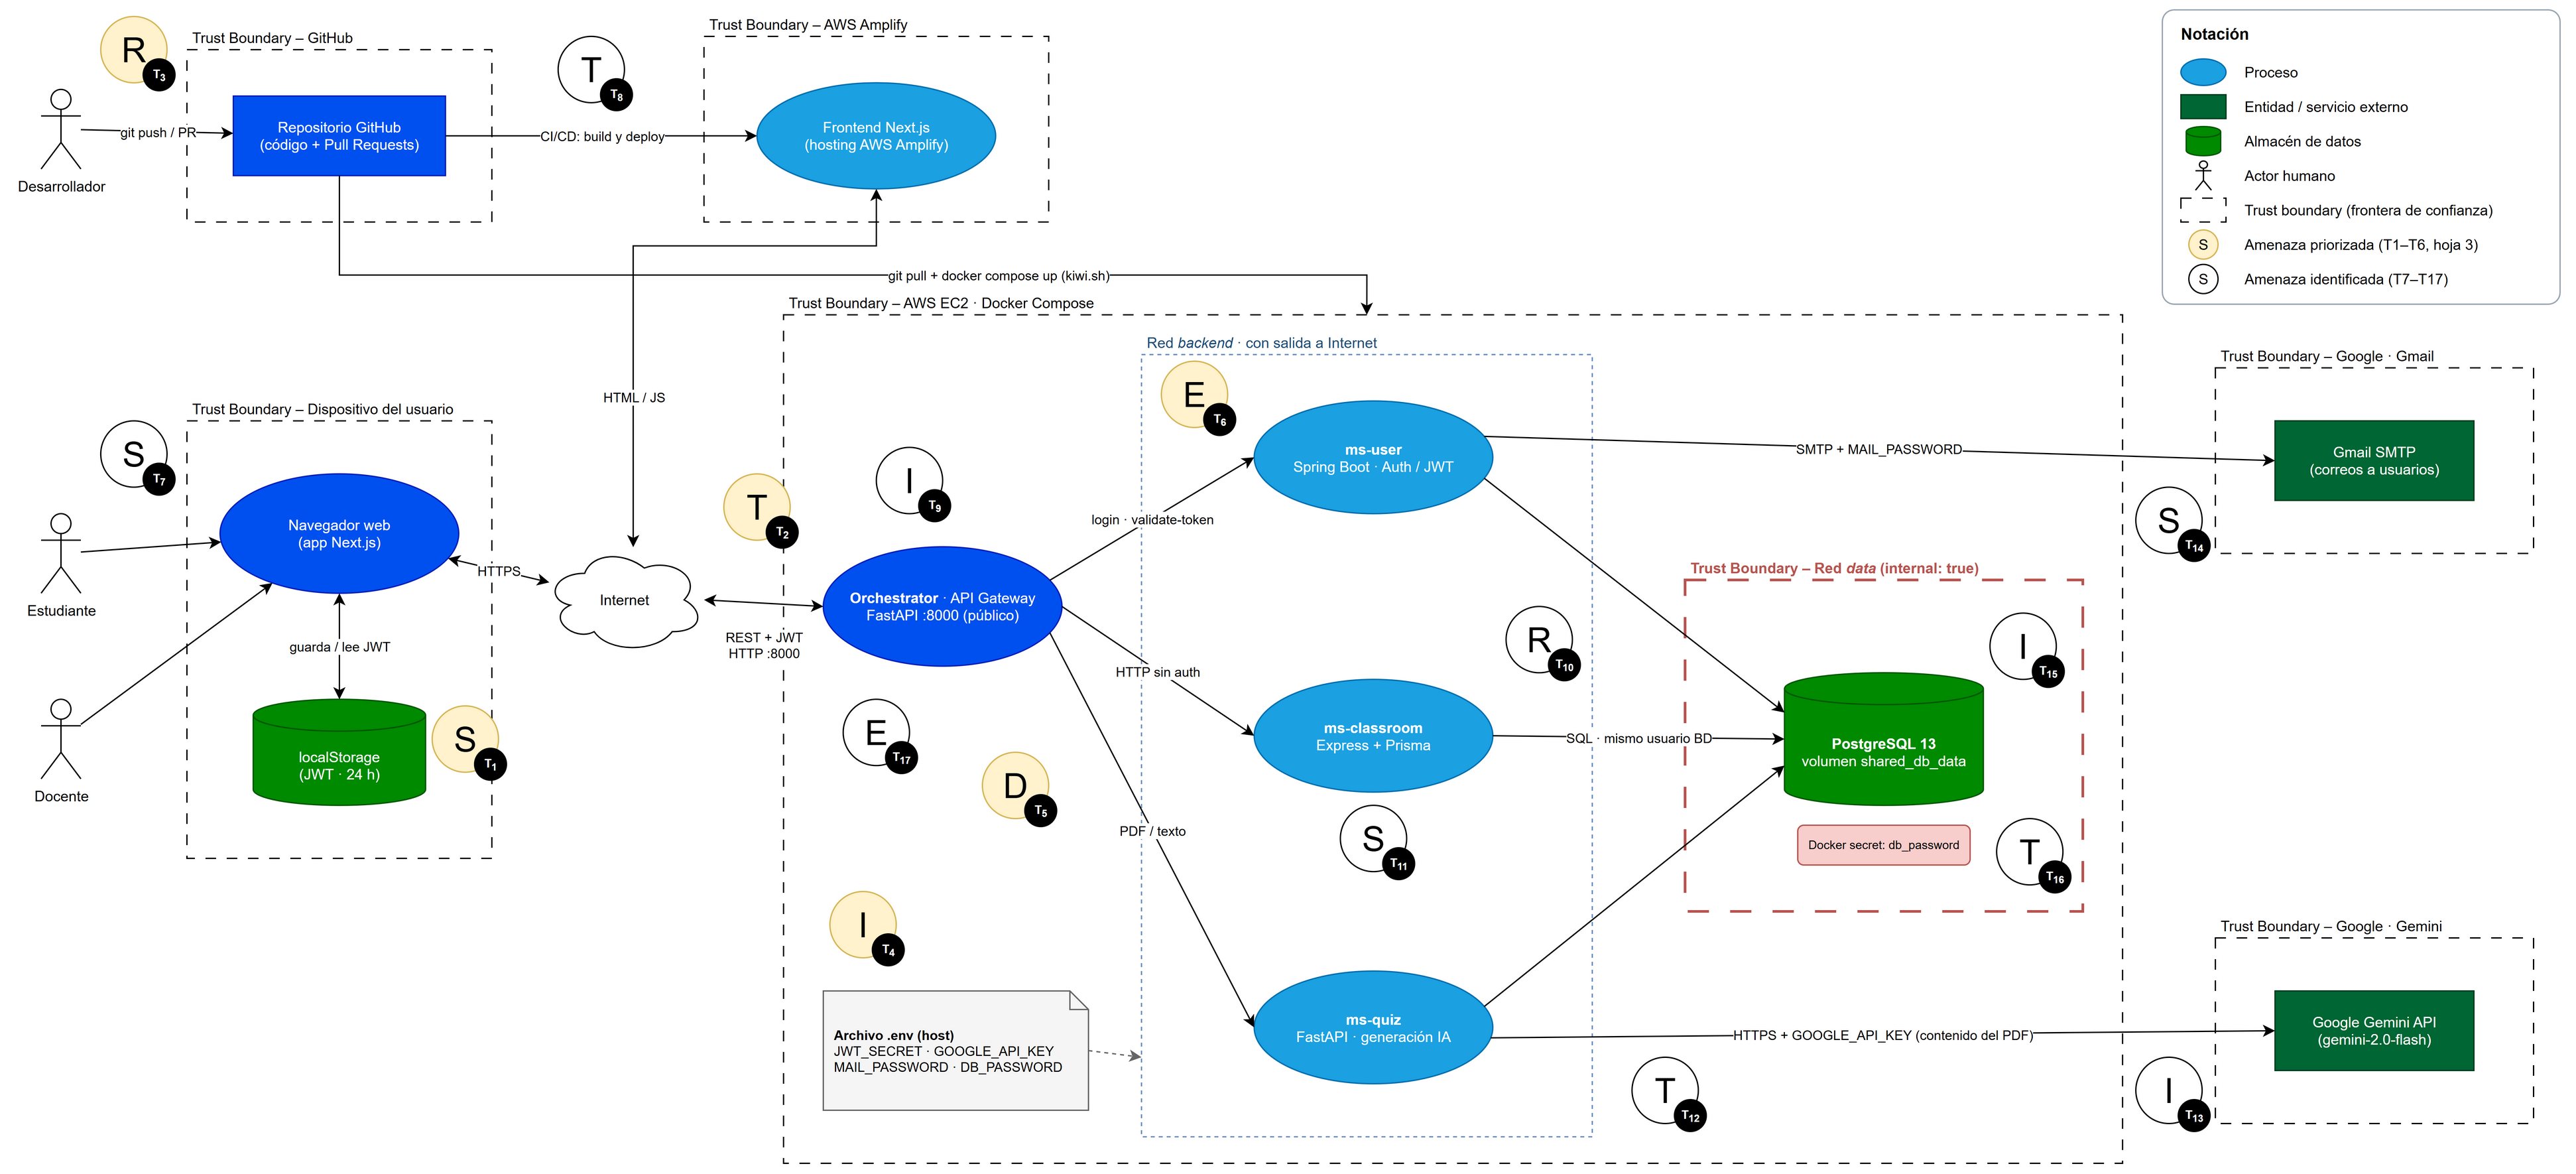
\includegraphics[width=0.95\linewidth]{stride-amenazas.png}};\end{tikzpicture}
    \column{0.26\textwidth}
    \statdark{0.86\linewidth}{17}{amenazas}\par\vskip3pt
    \stat{0.86\linewidth}{7}{fronteras}\par\vskip3pt
    \stat{0.86\linewidth}{6}{priorizadas}\par\vskip3pt
    
\begin{tikzpicture}\node[fill=soft,rounded corners=4pt,inner sep=6pt,text width=0.86\linewidth]{
      \tiny Una por categoría STRIDE (T1–T6), evaluadas con la plantilla del curso.};\end{tikzpicture}
  \end{columns}
\end{frame}

% ---------------------------------------------------------------- 4. Priorizadas
\begin{frame}{Seis amenazas priorizadas}{Amenazas priorizadas}
  \vskip2pt
  \begin{tabla}{L{3.6cm}L{2.4cm}L{2.6cm}Y}
    \thead{Amenaza} & \thead{Inherente} & \thead{Residual} & \thead{Estado en el cierre}\\
    T1 Spoofing · JWT en navegador & \cellcolor{amber}4 - High & 3 - Moderate & Pendiente: cookie HttpOnly y MFA\\
    T2 Tampering · HTTP sin TLS & 3 - Moderate & 3 - Moderate & Pendiente: proxy con TLS y HSTS\\
    T3 Repudiation · commits sin firma & \cellcolor{amber}4 - High & 3 - Moderate & Pendiente: firma y protección de main\\
    T4 Info. Disclosure · secretos & \cellcolor{amber}4 - High & \cellcolor{amber}4 - High & Parcial: árbol limpio, 46 JWT en historial\\
    T5 DoS · PDF y cuota IA & 3 - Moderate & 3 - Moderate & Parcial: 5 MB y 30 páginas; falta cuota\\
    T6 Elevation · rol docente & \cellcolor{amber}4 - High & \cellcolor{amber}4 - High & \cellcolor{okgreen}Mitigado: invitación validada\\
  \end{tabla}
  \vskip6pt
  {\tiny\color{muted} Plantilla evaluada sobre la línea base; estado verificado en main. T17 (IDOR) mitigada en rutas cubiertas.}
\end{frame}

% ---------------------------------------------------------------- 5. Pipeline
\begin{frame}{Pipeline de integración y distribución}{Pipeline CI/CD}
  \vskip4pt
  \begin{columns}[T]
    \column{0.68\textwidth}
    \begin{tikzpicture}\node[fill=white,draw=soft,rounded corners=4pt,inner sep=4pt]{%
      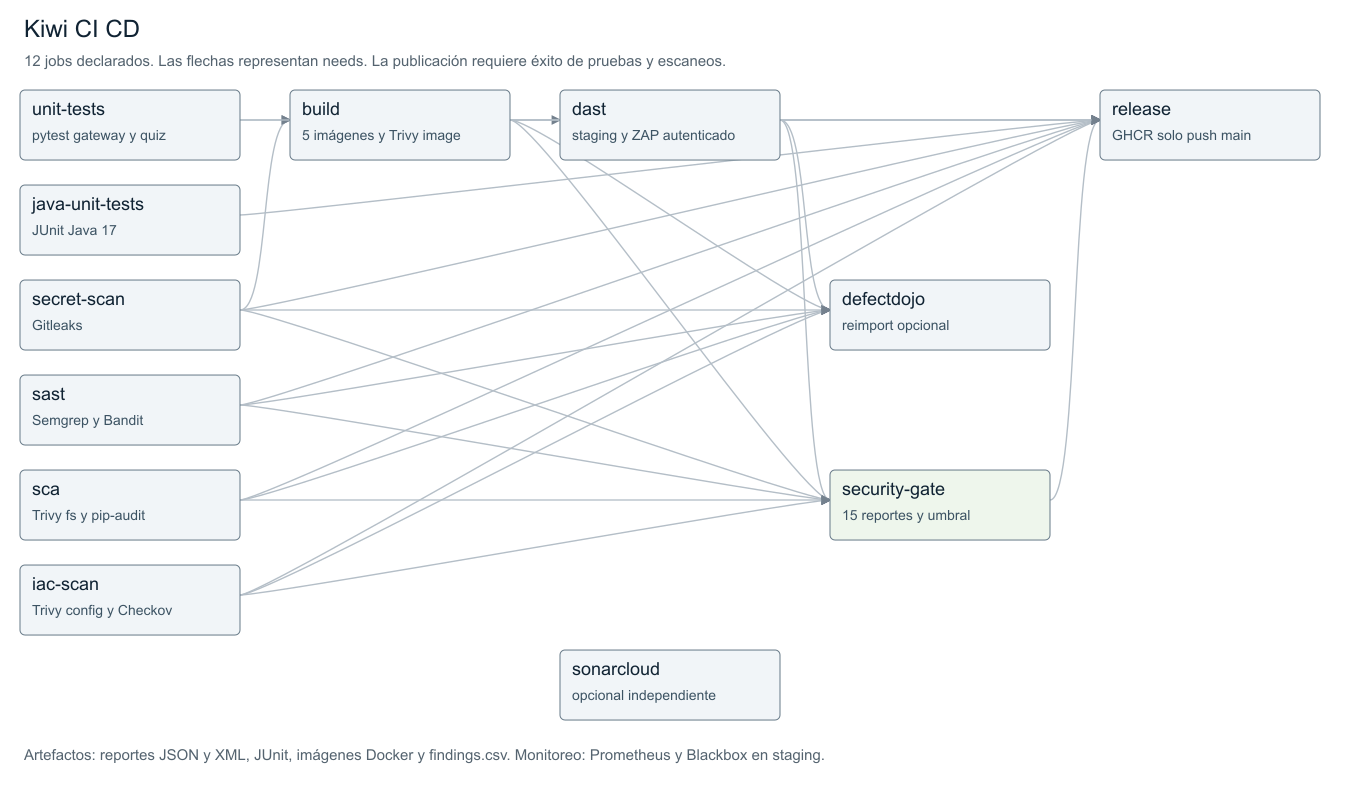
\includegraphics[width=0.95\linewidth]{pipeline-grafo.png}};\end{tikzpicture}
    \column{0.3\textwidth}
    \darkcard{0.86\linewidth}{%
      {\color{cyan}\tiny\bfseries COMPUERTA DE SEGURIDAD}\par\vskip6pt
      {\Large\bfseries CRITICAL por defecto.}\par\vskip8pt
      \scriptsize Sin sesión ZAP o sin los 15 reportes completos, la validación falla.
      12 jobs; GHCR solo con push a main.}
  \end{columns}
\end{frame}

% ---------------------------------------------------------------- 6. Herramientas
\begin{frame}{Herramientas y evidencias de seguridad}{Controles automatizados}
  \vskip10pt
  \begin{tabla}{L{3.2cm}L{4.4cm}Y}
    \thead{Control} & \thead{Herramientas} & \thead{Evidencia}\\
    \textbf{SAST} & Semgrep y Bandit & JSON y job de CI\\
    \textbf{DAST} & OWASP ZAP autenticado & API y frontend en staging\\
    \textbf{Secret scanning} & Gitleaks & Historial completo redactado\\
    \textbf{SCA e imágenes} & Trivy y pip-audit & Dependencias y 5 imágenes\\
    \textbf{IaC} & Checkov y Trivy config & Dockerfiles y configuración\\
  \end{tabla}
\end{frame}

% ---------------------------------------------------------------- 7. Mitigaciones
\begin{frame}{Mitigaciones comprobadas}{Mitigaciones}
  \vskip6pt
  \begin{columns}[T]
    \column{0.48\textwidth}
    \card{0.9\linewidth}{{\bfseries Roles e identidad}\par\vskip3pt\scriptsize
      \begin{itemize}\item Invitación docente (T6) y rechazo de IDs ajenos (T17).
      \item Perfiles sin hash de contraseña.\item PATCH actualiza solo campos permitidos.\end{itemize}}
    \column{0.48\textwidth}
    \card{0.9\linewidth}{{\bfseries Archivos y dependencias}\par\vskip3pt\scriptsize
      \begin{itemize}\item PDF con límite de tamaño y páginas (T5).
      \item Spring Boot 4.0.10 y Tomcat 11.0.27.\item Cero CRITICAL en el corte de CI.\end{itemize}}
  \end{columns}
  \vskip8pt
  \centering
  
\begin{tikzpicture}\node[fill=navy,rounded corners=4pt,inner sep=9pt,text width=0.9\textwidth,text=white]{
    {\color{cyan}\huge\bfseries 53}\enspace pruebas automatizadas\hfill
    {\color{cyan}\huge\bfseries 16}\enspace comprobaciones E2E locales correctas};\end{tikzpicture}
\end{frame}

% ---------------------------------------------------------------- 8. DefectDojo
\begin{frame}{Centralización en DefectDojo}{Gestión de hallazgos}
  \vskip2pt
  \begin{columns}[T]
    \column{0.4\textwidth}
    \centering
    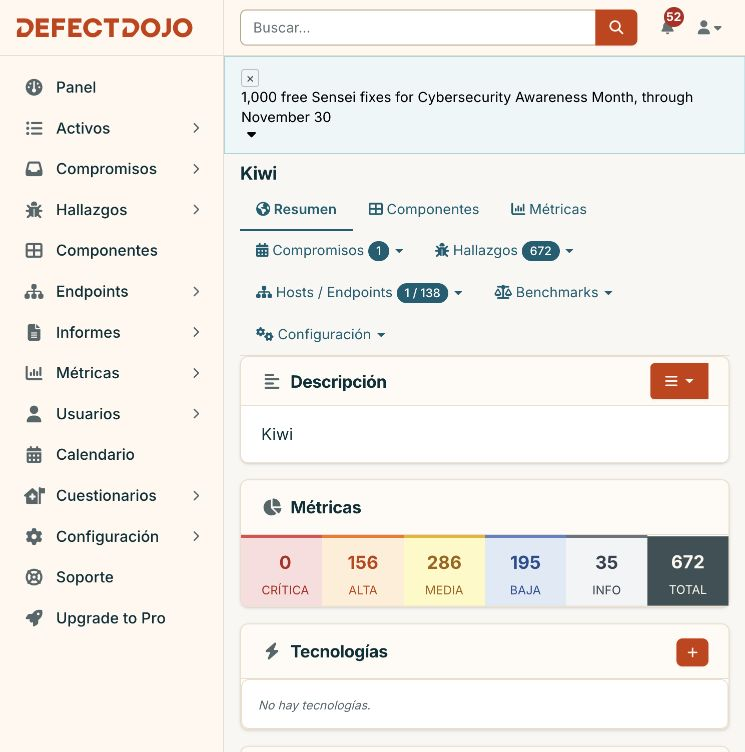
\includegraphics[height=0.72\textheight]{defectdojo-cierre.png}
    \column{0.56\textwidth}
    \stat{0.38\linewidth}{15}{tests conservados}\hfill\stat{0.38\linewidth}{561}{mitigados}\par\vskip4pt
    \stat{0.38\linewidth}{36}{nuevos}\hfill\statdark{0.38\linewidth}{672}{activos}\par\vskip4pt
    
\begin{tikzpicture}\node[fill=soft,rounded corners=4pt,inner sep=6pt,text width=0.92\linewidth]{
      \scriptsize\textbf{Corte CI 45067822680.} Instancia propia local. Línea base importada:
      1197 hallazgos, 33 críticos.};\end{tikzpicture}
  \end{columns}
\end{frame}

% ---------------------------------------------------------------- 9. Resultados
\begin{frame}{Detecciones antes y después}{Resultados}
  \begin{columns}[T]
    \column{0.64\textwidth}
    \begin{tikzpicture}
      \begin{axis}[ybar, bar width=11pt, width=\linewidth, height=0.62\textheight,
        symbolic x coords={CRITICAL,HIGH,MEDIUM,LOW,INFO}, xtick=data,
        ymin=0, ymax=540, area legend, axis lines*=left, ytick=\empty, axis y line=none,
        nodes near coords, every node near coord/.append style={font=\tiny},
        tick label style={font=\tiny}, legend style={font=\tiny,draw=none,fill=none,
        at={(0.5,-0.18)},anchor=north,legend columns=2}, enlarge x limits=0.15]
        \addplot[fill=muted!50,draw=none] coordinates {(CRITICAL,33) (HIGH,382) (MEDIUM,485) (LOW,275) (INFO,23)};
        \addplot[fill=cyan,draw=none] coordinates {(CRITICAL,0) (HIGH,156) (MEDIUM,286) (LOW,194) (INFO,36)};
        \legend{Inicial CI, Cierre CI}
      \end{axis}
    \end{tikzpicture}
    \column{0.32\textwidth}
    \darkcard{0.86\linewidth}{%
      {\color{cyan}\Large\bfseries 1198 a 672}\par\vskip6pt
      {\Large\bfseries 43,9\,\%}\par{\scriptsize menos detecciones}\par\vskip6pt
      {\Large\bfseries 62,4\,\%}\par{\scriptsize menos CRITICAL y HIGH}}\par\vskip3pt
    
\begin{tikzpicture}\node[fill=soft,rounded corners=4pt,inner sep=6pt,text width=0.86\linewidth]{
      \tiny Confirmado en main (run 45104881204): 672 y 0 CRITICAL. Cobertura y bases de
      vulnerabilidades limitan la comparación.};\end{tikzpicture}
  \end{columns}
\end{frame}

% ---------------------------------------------------------------- 10. Ambientes
\begin{frame}{Ambientes y monitoreo}{Ambientes y monitoreo}
  \vskip4pt
  \begin{columns}[T]
    \column{0.58\textwidth}
    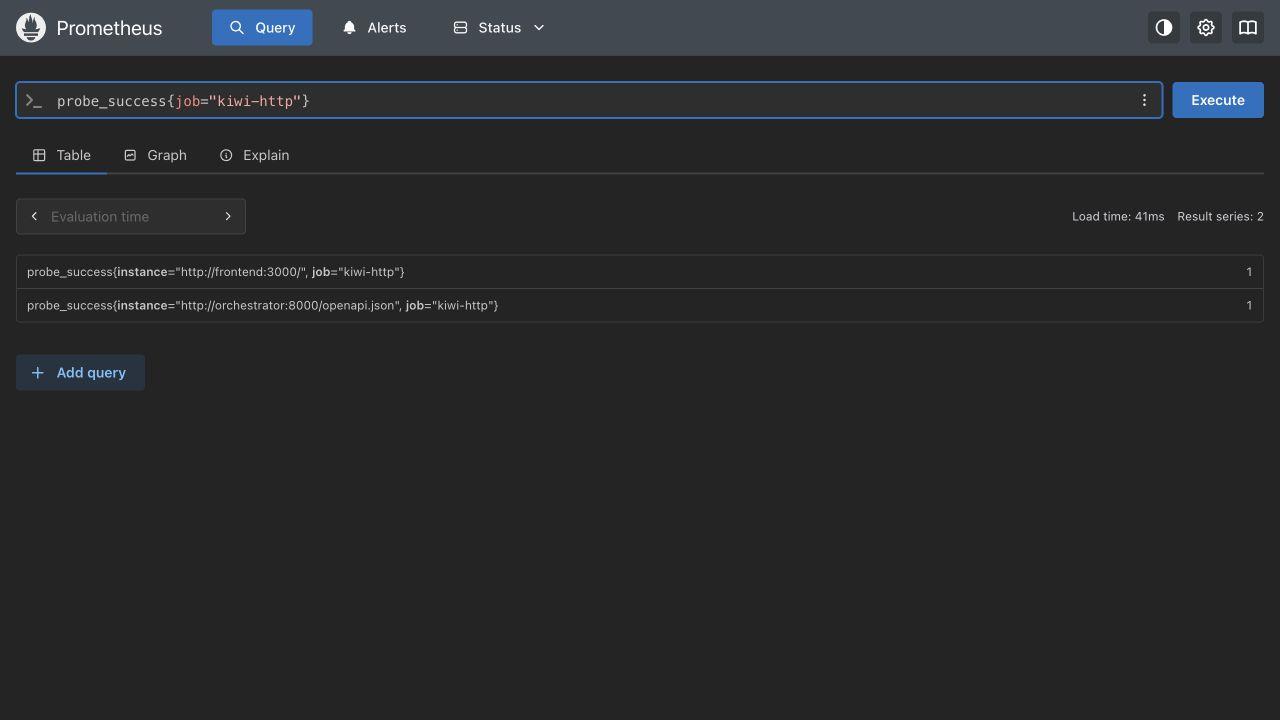
\includegraphics[width=\linewidth]{prometheus-sondas.png}
    \column{0.4\textwidth}
    \card{0.88\linewidth}{\small\num{1}\enspace Desarrollo local\par\vskip4pt
      \num{2}\enspace Staging efímero en CI\par\vskip4pt
      \num{3}\enspace Distribución en GHCR}\par\vskip3pt
    \darkcard{0.88\linewidth}{{\color{cyan}\tiny\bfseries ESTADO}\par\vskip2pt\scriptsize
      \begin{itemize}\item Dos sondas HTTP sanas.\item Alerta y recuperación probadas.
      \item GHCR: 4 de 5 imágenes; frontend rechazada.\item Producción por desplegar.\end{itemize}}
  \end{columns}
\end{frame}

% ---------------------------------------------------------------- 11. SAMM
\begin{frame}{Madurez según OWASP SAMM}{Madurez OWASP SAMM}
  \vskip10pt
  \begin{tabla}{L{3.6cm}L{5.0cm}Y}
    \thead{Práctica} & \thead{Evidencia} & \thead{Límite}\\
    \textbf{Threat Assessment} & STRIDE con 17 amenazas y DFD & Revisión periódica pendiente\\
    \textbf{Secure Build} & Build y análisis automatizados & Tags y reglas externas mutables\\
    \textbf{Defect Management} & Reimportación en DefectDojo & Decisiones de riesgo pendientes\\
    \textbf{Security Testing} & Herramientas y pruebas negativas & Nivel 1 en alcance revisado\\
    \textbf{Incident Management} & Sondas y alerta comprobada & Sin operación productiva sostenida\\
  \end{tabla}
\end{frame}

% ---------------------------------------------------------------- 12. Cierre
\begin{frame}{Lecciones y siguientes decisiones}{Cierre}
  \vskip6pt
  \begin{columns}[T]
    \column{0.56\textwidth}
    \card{0.92\linewidth}{{\bfseries Lecciones}\par\vskip6pt\small
      \num{1}\enspace La sesión autenticada de ZAP encontró el hash.\par\vskip6pt
      \num{2}\enspace Un job verde puede haber omitido herramientas.\par\vskip6pt
      \num{3}\enspace STRIDE encontró fallos que ningún escáner reportaba.}
    \column{0.4\textwidth}
    \darkcard{0.88\linewidth}{{\color{cyan}\bfseries Siguientes decisiones}\par\vskip3pt\scriptsize
      \begin{itemize}
      \item PR \#11, \#12 y \#13 integrados; CI en main con 0 CRITICAL.
      \item Corregir permisos de \texttt{kiwi-frontend} en GHCR.
      \item Confirmar rotación de JWT en el equipo y revisar 156 HIGH.
      \item Cerrar T1--T5: cookies, TLS, firma, secretos y cuotas.
      \end{itemize}}
  \end{columns}
\end{frame}

\end{document}
